\documentclass{beamer}
\usetheme{Madrid}

\usepackage{amsmath, amssymb, amsthm}
\usepackage{graphicx}
\usepackage{listings}
\usepackage{gensymb}
\usepackage[utf8]{inputenc}
\usepackage{hyperref}
\usepackage{tikz}
\lstset{
	language=Python,
	basicstyle=\ttfamily\small,
	keywordstyle=\color{blue},
	stringstyle=\color{orange},
	numbers=left,
	numberstyle=\tiny\color{gray},
	breaklines=true,
	showstringspaces=false
}
\usetikzlibrary{decorations.pathmorphing}

\title{Question-12.9.ex.19}
\author{EE24BTECH11030 - J.KEDARANANDA}
\date{}
\begin{document}
	
	\frame{\titlepage}
	
	\begin{frame}
		\frametitle{Question}
		Solve the differential equation:
		
		$y' = y + \cos x$
	\end{frame}
	
	\begin{frame}
		\frametitle{Theoritical Solution : }
		
		\centering
		The given differential equation is a first-order linear ordinary differential equation. Let $y(0) = c_1$. By the definition of the Laplace transform,
		
		\[
		\mathcal{L}(f(t)) = \int_0^\infty e^{-st} f(t) \, dt
		\]
		
		Some used properties of the Laplace transform include:
		\begin{align}
			\mathcal{L}(f'(t)) &= s\mathcal{L}(f(t)) - f(0) \\
			\mathcal{L}(cf(t)) &= c\mathcal{L}(f(t)) \\
			\mathcal{L}(e^{at}f(t)) &= F(s - a), \quad \text{where } F(s) = \mathcal{L}(f(t)) \\
			\mathcal{L}(\cos x) &= \frac{s}{s^2 + 1}
		\end{align}
	\end{frame}
	\begin{frame}{Applying the Laplace Transform}
		\textbf{Applying the Laplace transform to the given differential equation:}
		
		\[
		y' - y = \cos x
		\]
		
		Take the Laplace transform on both sides:
		
		\begin{align}
			\mathcal{L}(y') - \mathcal{L}(y) &= \mathcal{L}(\cos x)
		\end{align}
		
		Using the properties of the Laplace transform:
		
		\begin{align}
			(s\mathcal{L}(y) - y(0)) - \mathcal{L}(y) &= \frac{s}{s^2 + 1}
		\end{align}
		
		Let $\mathcal{L}(y) = Y(s)$. Substituting $y(0) = c_1$, we get:
		
		\begin{align}
			sY(s) - c_1 - Y(s) &= \frac{s}{s^2 + 1}
		\end{align}
	\end{frame}
	\begin{frame}
		Simplify:
		
		\begin{align}
			(s - 1)Y(s) &= c_1 + \frac{s}{s^2 + 1} \\
			Y(s) &= \frac{c_1}{s - 1} + \frac{s}{(s^2 + 1)(s - 1)}
		\end{align}
		\textbf{Partial fraction decomposition:}
		
		For $\frac{s}{(s^2 + 1)(s - 1)}$, decompose into:
		
		\begin{align}
			\frac{s}{(s^2 + 1)(s - 1)} &= \frac{A}{s - 1} + \frac{Bs + C}{s^2 + 1}
		\end{align}
		
		Solve for $A$, $B$, and $C$ by equating numerators:
		
		\begin{align}
			s &= A(s^2 + 1) + (Bs + C)(s - 1)
		\end{align}
	\end{frame}
	\begin{frame}{Partial fraction decomposition:}
		Equating coefficients:
		
		\begin{align}
			A + B &= 0 \quad \text{(coefficient of $s^2$)} \\
			-B + C &= 1 \quad \text{(coefficient of $s$)} \\
			A - C &= 0 \quad \text{(constant term)}
		\end{align}
		
		The partial fraction decomposition becomes:
		
		\begin{align}
			\frac{s}{(s^2 + 1)(s - 1)} &= \frac{\frac{1}{2}}{s - 1} + \frac{-\frac{1}{2}s + \frac{1}{2}}{s^2 + 1}
		\end{align}
	\end{frame}
	\begin{frame}
		\textbf{Rewrite $Y(s)$:}
		
		\begin{align}
			Y(s) &= \frac{c_1}{s - 1} + \frac{\frac{1}{2}}{s - 1} + \frac{-\frac{1}{2}s + \frac{1}{2}}{s^2 + 1}
		\end{align}
		
		Combine terms:
		
		\begin{align}
			Y(s) &= \frac{c_1 + \frac{1}{2}}{s - 1} - \frac{\frac{1}{2}s}{s^2 + 1} + \frac{\frac{1}{2}}{s^2 + 1}
		\end{align}
	\end{frame}
	\begin{frame}{Final Solution}
		\textbf{Final solution:}
		
		\begin{align}
			y(x) &= \left(c_1 + \frac{1}{2}\right)e^x - \frac{1}{2}\cos x + \frac{1}{2}\sin x
		\end{align}
	\end{frame}
	\begin{frame}{Computational Solution: Bilinear (sim2)}
		\textbf{Computational Solution Bilinear (sim2):}
		
		We use the bilinear $z$-transform:
		
		\begin{align}
			s &= \frac{2}{T} \frac{1 - z^{-1}}{1 + z^{-1}}.
		\end{align}
		
		The total $Y(z)$ is:
		
		\begin{align}
			Y(z) &= 
			\left(c_1 + \frac{1}{2}\right) \cdot 
			\frac{1 + z^{-1}}{\frac{2}{T} - 1 - \left(\frac{2}{T} + 1\right)z^{-1}} \\
			&\quad - \frac{\frac{1}{T} (1 - z^{-1})}{\left(\frac{2}{T}\right)^2 (1 - z^{-1})^2 + (1 + z^{-1})^2} \\
			&\quad + \frac{\frac{1}{2} (1 + z^{-1})^2}{\left(\frac{2}{T}\right)^2 (1 - z^{-1})^2 + (1 + z^{-1})^2}
		\end{align}
	\end{frame}
	\begin{frame}{Computational Solution: Extended Steps}
		\begin{align}
			&\Bigg(
			\left(\frac{2}{T}\right)^2 \left(1 - z^{-1}\right)^2 + \left(1 + z^{-1}\right)^2
			\Bigg)^{-1} 
			\Bigg[
			\left(\frac{2}{T} - 1\right) - \left(\frac{2}{T} + 1\right)z^{-1} 
			\Bigg] Y(z) \nonumber \\
			&\quad = f(z^{-1}, z^{-2}, z^{-3}) + c
		\end{align}
		
		\begin{align}
			&\Bigg(
			\left(\frac{4}{T^2} + 1\right) + \left(2 - \frac{8}{T^2}\right)z^{-1} + \left(\frac{4}{T^2} + 1\right)z^{-2} 
			\Bigg) 
			\Bigg(\frac{2}{T} - 1 - \left(\frac{2}{T} + 1\right)z^{-1}\Bigg) Y(z) \nonumber \\
			&\quad = f(z^{-1}, z^{-2}, z^{-3}) + c
		\end{align}
		\begin{align}
			\left(a + bz^{-1} + cz^{-2}\right) \left(d + ez^{-1}\right) Y(z) = f(z^{-1}, z^{-2}, z^{-3}) + c
		\end{align}
	\end{frame}
	\begin{frame}{Computational Solution: Extended Steps}
		\begin{align}
			&adY(z) + (ae+bd)z^{-1}Y(z) + (cd+be)z^{-2}Y(z) + ce z^{-3}Y(z) \nonumber \\
			&\quad = f(z^{-1}, z^{-2}, z^{-3}) + c
		\end{align}
		
		\begin{align}
			\text{where } 
			a &= \left(\frac{4}{T^2}+1\right), \, 
			b = \left(2-\frac{8}{T^2}\right), \, 
			c = \left(\frac{4}{T^2}+1\right), \, \nonumber 
			d = \frac{2}{T}-1, \, 
			e = -\left(\frac{2}{T}+1\right)
		\end{align}
		
		\begin{align}
			&\rightarrow 
			adz^{3}Y(z) + (ae+bd)z^{2}Y(z) + (cd+be)z^{1}Y(z) + ceY(z) \nonumber \\
			&\quad = f'(z^{1}, z^{2}, z^{3}) + c
		\end{align}
		\begin{align}
			&\rightarrow 
			ady[n+3] + (ae+bd)y[n+2] + (cd+be)y[n+1] + cey[n] \nonumber \\
			&\quad = f''(\delta[n], \delta[n+1], \delta[n+2], \delta[n+3])
		\end{align}
	\end{frame}
	\begin{frame}{Computational Solution: Extended Steps}
		\begin{align}
			\text{Given: } y[0] = c_{1}, \, y[1] &= y[0] + h y'[0]
		\end{align}
		
		\begin{align}
			y[1] &= c_{1} + h(1+a)
		\end{align}
		
		\begin{align}
			y[2] &= y[1] + h(y'[1])
		\end{align}
		
		\begin{align}
			y[2] &= y[1] + h(y[1] + \cos(h))
		\end{align}
		
		\begin{align}
			y[3] &= y[2] + h(y[2] + \cos(2h))
		\end{align}
		
		\begin{align}
			n \geq 1 \rightarrow \delta[n], \delta[n+1], \delta[n+2], \delta[n+3] &= 0
		\end{align}
		
		\begin{align}
			\text{Difference equation: } 
			y[n+3] &= -\frac{1}{ad} \left[(ae+bd)y[n+2] + (cd+be)y[n+1] + cey[n]\right]
		\end{align}
	\end{frame}
	\begin{frame}{Difference Equation}
		\begin{align}
			\text{Difference equation: } 
			y[n+3] &= -\frac{1}{ad} \left[(ae+bd)y[n+2] + (cd+be)y[n+1] + cey[n]\right]
		\end{align}
	\end{frame}
	\begin{frame}{Computational Solution: Trapezoid Method}
		\textbf{Computational Solution: Trapezoid Method: (sim1)}
		
		\subsection*{Step 1: Transform the DE into a First-Order System}
		
		The given differential equation is already in first-order form:
		$\frac{dy}{dx} = y + \cos x$.
		
		Let:
		$y = y_1$, so $\frac{dy_1}{dx} = y_1 + \cos x$.
		
		\subsection*{Step 2: Apply the Trapezoidal Rule}
		
		Using the Trapezoidal Rule, the equation can be written as:
		\begin{align}
			y_{n+1} - y_n &= \frac{h}{2} \big( (y_n + \cos x_n) + (y_{n+1} + \cos x_{n+1}) \big),
		\end{align}
		where $h$ is the step size, $y_n$ is the value of $y$ at $x_n$, and $y_{n+1}$ is the value of $y$ at $x_{n+1} = x_n + h$.
		
		\subsection*{Step 3: Solve for $y_{n+1}$}
		
		Rearranging Equation (1) to isolate $y_{n+1}$:
		\begin{align}
			y_{n+1} - \frac{h}{2} y_{n+1} &= y_n + \frac{h}{2} (y_n + \cos x_n + \cos x_{n+1}), \\
			y_{n+1} \big( 1 - \frac{h}{2} \big) &= y_n \big( 1 + \frac{h}{2} \big) + \frac{h}{2} (\cos x_n + \cos x_{n+1}),
		\end{align}
	\end{frame}
	\begin{frame}{Computational Solution: Trapezoid Method (Continued)}
		\subsection*{Step 3: Solve for $y_{n+1}$}
		
		\begin{align}
			y_{n+1} &= \frac{y_n \big( 1 + \frac{h}{2} \big) + \frac{h}{2} (\cos x_n + \cos x_{n+1})}{1 - \frac{h}{2}}.
		\end{align}
		
		\subsection*{Step 4: Iterative Scheme}
		
		The final iterative formula is:
		\begin{align}
			y_{n+1} &= \frac{y_n \big( 1 + \frac{h}{2} \big) + \frac{h}{2} (\cos x_n + \cos x_{n+1})}{1 - \frac{h}{2}}.
		\end{align}
		
		\subsection*{Step 5: Initial Conditions and Computation}
		
		Given the initial condition:
		$x_0 = 0$, $y_0 = 0$,
		and a chosen step size $h$, the values of $y_n$ can be iteratively computed for subsequent $x_n$.\\
	\end{frame}
	
	\begin{frame}
		\frametitle{Diagram}
		\begin{figure}[!ht]
			\centering
			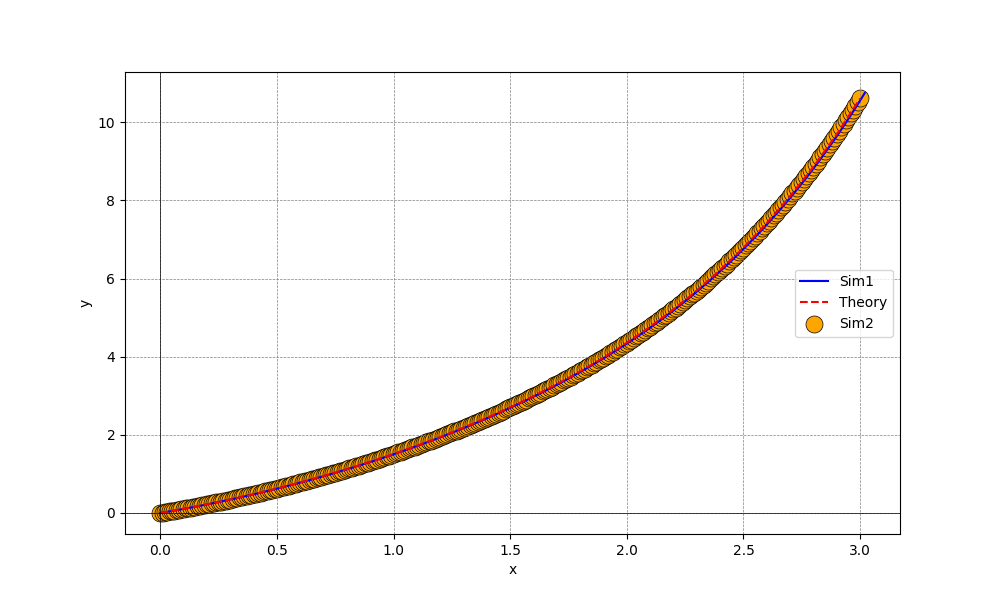
\includegraphics[width=\linewidth]{figs/Fig.png}
		\end{figure}
	\end{frame}
\end{document}

